\section{实验设计}

本实验系统由四个主要模块组成:Hamming 编解码、交织与解交织、QPSK 调制解调以及加性高斯白噪声(AWGN)信道。这些模块协同工作,模拟实际通信系统中的信号处理与传输过程。

\subsection{Hamming 编解码}



\subsection{交织与解交织}



\subsection{QPSK 调制解调}

在现代数字通信系统中,QPSK(Quadrature Phase Shift Keying,正交相位调制)是一种高效的调制方式,它通过在同一时间内传输两个比特来实现高数据传输率。如图 \ref{fig:qpsk_model} 所示,QPSK 调制器将输入的二进制数据分成两部分,每部分表示一个信号的相位,分别控制正交的两个载波(I路和Q路)。这种方式可以有效利用带宽,同时保持较高的抗干扰能力。

\begin{figure}[ht]
    \centering
    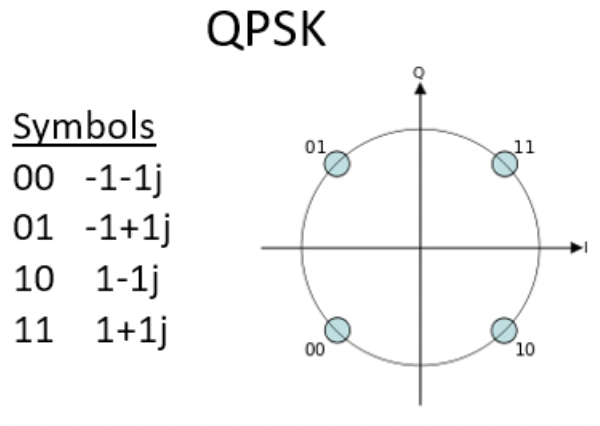
\includegraphics[width=.3\textwidth]{static/qpsk_model.png}
    \caption{QPSK 调制解调模型}
    \label{fig:qpsk_model}
\end{figure}

QPSK 调制与解调过程包括以下几个步骤:

\begin{itemize} 
    \item 调制过程:输入的数据每两位作为一个信号符号,映射到四个不同的相位上,通常是 $0^\circ$,$90^\circ$,$180^\circ$ 和 $270^\circ$,分别对应不同的比特组合。
    \item 解调过程:接收端根据信号的相位变化来恢复发送的比特流。通过比较接收到的信号与阈值,判断其属于哪个相位,并输出对应的比特组合。
\end{itemize}





\subsection{AWGN 信道模型}

AWGN(Additive White Gaussian Noise,加性白噪声)信道模型广泛应用于无线通信领域,用于模拟理想情况下的噪声影响。在此信道模型中,噪声是加性、均匀分布的,且具有高斯分布特性。在本实验中,AWGN 信道的模拟过程分为两个步骤:首先,通过 LFSR(线性反馈移位寄存器)生成伪随机数序列;然后,利用 Box-Muller 变换将这些伪随机数转换为服从高斯分布的随机数,最终将这些噪声加到信号中,模拟实际通信中的噪声干扰。

\subsubsection{LFSR}

为了产生 Gaussian 白噪声,首先需要生成均匀分布的伪随机数序列。本实验中,我们采用线性反馈移位寄存器(LFSR),通过移位寄存器和特定的反馈函数来生成这些随机数。

图 \ref{fig:lfsr_model} 展示了一个 16 位 Fibonacci LFSR。其采用的特征多项式为 $X^{16} + X^{14} + X^{13} + X^{11} + 1$。该多项式确保了生成的随机序列的周期最大(65535,不包括全零状态),以有效地模拟随机性。移位寄存器逐位输出随机序列的每一位,同时通过反馈机制决定下一个状态。这一过程不断重复,直到达到最大周期。例如,图中的状态为 0xACE1 (十六进制) ,下一个状态是 0x5670.

\begin{figure}[ht]
    \centering
    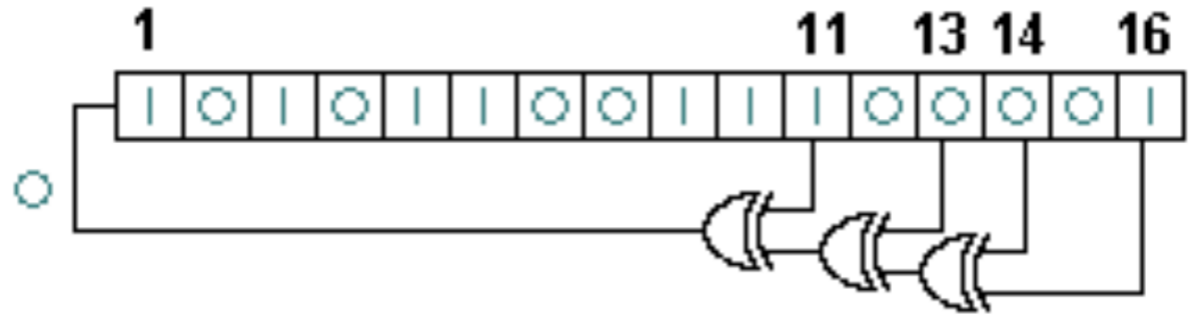
\includegraphics[width=.6\textwidth]{static/lfsr_model.png}
    \caption{一个 16-位 Fibonacci LFSR}
    \label{fig:lfsr_model}
\end{figure}

\subsubsection{Box-Muller}

Box-Muller 变换是一种用于从均匀分布的随机数生成高斯分布随机数的方法。在本实验中,我们首先生成两个均匀分布的随机数 $U_1, U_2 \sim U(0, 1)$,然后通过以下公式将其转换为符合标准正态分布的随机数:

$$
\begin{aligned}
X = \sqrt{-2\ln U_1} \cos(2\pi U_2) \\
Y = \sqrt{-2\ln U_1} \sin(2\pi U_2)
\end{aligned}
$$

其中,$X$ 和 $Y$ 分别为符合标准正态分布的随机变量。
